\textbf{Beispiel 1}\\ \\
a)\\ \\
Wirkende Kräfte
\begin{figure}[h]
		\centering
		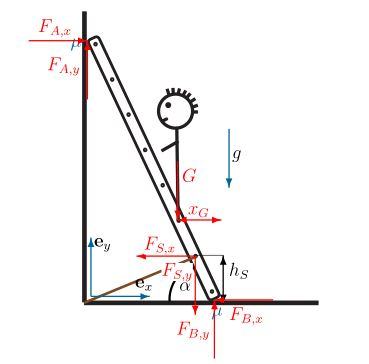
\includegraphics[width=8cm]{tikz/08_07_2016_1a}
\end{figure}
\newline
b)\\ \\
Kräftegleichgewicht:
\begin{align*}
	\textbf{e}_x &: F_{A,x} - F_{B,x} = 0 \\
	\textbf{e}_y &: F_{A,y} + F_{B,y} - G = 0 \quad,G = mg
\end{align*}
Momentengleichgewicht im Fußende der Leiter:
\[
	x_G G - L\cos\alpha F_{A,y} - L\sin\alpha F_{A,x} = 0
\]
c)\\ \\
Die beiden Haftbedingungen lauten 
\begin{align*}
	F_{A,y} &\leq \mu F_{A,x} \\
	F_{B,x} &\leq \mu F_{B,y}
\end{align*}
Setzt man diese in die Gleichungen des Kräftegleichfewichts ein erhält man die Teilkräfte. Anfangs müssen aber noch einige Zwischenrechnungen durchgeführt werden.
\begin{align*}
	F_{A,y} = \mu F_{A,x} &\qquad F_{B,x} = \mu F_{B,y} \\
	F_{A,x} &= F_{B,x} \\
	F_{A,y} &= G - F_{B,y} \\
	\mu F_{A,x} &= G - F_{B,y} \\
	\mu^2 F_{B,y} &= G - F_{B,y} \\
	(\mu^2 + 1) F_{B,y} &= G \\
	F_{B,y} &= \frac{1}{\mu^2 + 1}G \\
	F_{B,x} = F_{A,x} &= \frac{\mu}{\mu^2 + 1} G \\
	F_{A,y} &= \frac{\mu^2}{\mu^2 + 1}
\end{align*}
i)\\ \\
Damit man die Leiter nicht wegrutscht muss
\begin{align*}
	x_G G - L\cos\alpha\frac{\mu^2}{\mu^2 + 1} G - L\sin\alpha\frac{\mu}{\mu^2 + 1} G \leq 0 \\
	x_G \leq L\frac{\mu}{\mu^2 + 1} (\sin\alpha + \mu \cos\alpha)
\end{align*}
ii)\\ \\
Folgende Bedingung gilt für den Steigungswinkel
\[
	\tan\alpha \geq \frac{1}{\mu}
\]
Daraus folgen folgende Grenzen für den Steigungswinkel
\[
	\frac{\pi}{2} \geq \alpha \geq \arctan\left(\frac{1}{\mu}\right)
\]
Aus der Angabe ist ersichtlich das der Steigungswinkel maximal $\frac{\pi}{2}$ sein kann. \\ \\
d)\\ \\
Adaptiertes Kräftegleichgewicht:
\begin{align*}
	F_{A,x} - \mu F_{B,y} - \cos\beta F_S &= 0 \\
	\mu F_{A,x} + F_{B,y} - \sin\beta F_S &= G \\5
	-(L\mu \cos\alpha + L\sin\alpha)F_{A,x} + &\left(\frac{\sin\beta}{\tan\beta} + \cos\beta\right)h_S F_S = -L\cos\alpha G
\end{align*}
\newpage
\noindent
Durch Umformen folgt die Seilkraft
\[
	F_S = G \frac{L\tan\alpha \cos\alpha (\mu^2 + 1)}{((a - h_S(\mu^2 + 1))\cos\beta + a\mu\sin\alpha)\tan\alpha - \sin\beta h_S(\mu^2 + 1)}
\]
mit
\[
	a = L(\sin\alpha + \mu \cos\alpha)
\]